%%% Přílohy k diplomové práci, existují-li (různé dodatky jako výpisy programů,
%%% diagramy apod.). Každá příloha musí být alespoň jednou odkazována z vlastního
%%% textu práce. Přílohy se číslují.
\chapwithtoc{Attachments}
\appendix

%% Uživatelská dokumentace
%\include{att1}
%
%% Programátorský průvodce & minimální demo
%\include{att2}
%
%% Obsah CD
%\include{att3}

\openright

%%%% att1.tex
\chapter{CD with the method}
\label{att:cd}
On this CD, we provide both the~source code of this method and a~stand-alone executable which demonstrates its functionality. See the~file readme.txt for more information.


\chapter{Results on a~reference image}
\label{att:res_ref}

This attachment demonstrates on a~reference heightmap how the~output of compression varies depending on the~chosen maximum deviation. On the~top, there will be always the~original image, in the~center, the~compressed one and on the~bottom, their difference in blue-to-yellow scale, with blue being the~minimum value and yellow being the~maximum value.

\newcommand{\incref}[1]{\includegraphics[width=0.5\textwidth]{#1}}

\begin{figure}
	\begin{center}
		\incref{figures/out_0.png} \\ \vspaceimg
		\incref{figures/out_0.png} \\ \vspaceimg
		\incref{figures/out_diff_0.png} \\ \vspaceimg
	\end{center}
	\caption{Maximum deviation 0.}
\end{figure}

\begin{figure}
	\begin{center}
		\incref{figures/out_0.png} \\ \vspaceimg
		\incref{figures/out_1.png} \\ \vspaceimg
		\incref{figures/out_diff_1.png} \\ \vspaceimg
	\end{center}
	\caption{Maximum deviation 1.}
\end{figure}

\begin{figure}
	\begin{center}
		\incref{figures/out_0.png} \\ \vspaceimg
		\incref{figures/out_2.png} \\ \vspaceimg
		\incref{figures/out_diff_2.png} \\ \vspaceimg
	\end{center}
	\caption{Maximum deviation 2.}
\end{figure}

\begin{figure}
	\begin{center}
		\incref{figures/out_0.png} \\ \vspaceimg
		\incref{figures/out_5.png} \\ \vspaceimg
		\incref{figures/out_diff_5.png} \\ \vspaceimg
	\end{center}
	\caption{Maximum deviation 5.}
\end{figure}

\begin{figure}
	\begin{center}
		\incref{figures/out_0.png} \\ \vspaceimg
		\incref{figures/out_10.png} \\ \vspaceimg
		\incref{figures/out_diff_10.png} \\ \vspaceimg
	\end{center}
	\caption{Maximum deviation 10.}
\end{figure}

\begin{figure}
	\begin{center}
		\incref{figures/out_0.png} \\ \vspaceimg
		\incref{figures/out_15.png} \\ \vspaceimg
		\incref{figures/out_diff_15.png} \\ \vspaceimg
	\end{center}
	\caption{Maximum deviation 15.}
\end{figure}

\begin{figure}
	\begin{center}
		\incref{figures/out_0.png} \\ \vspaceimg
		\incref{figures/out_20.png} \\ \vspaceimg
		\incref{figures/out_diff_20.png} \\ \vspaceimg
	\end{center}
	\caption{Maximum deviation 20.}
\end{figure}

%%%% Pro inline pdf
\chapter{The~paper}
\label{att:paper}

Hereby, we would like to include a~paper about this method written by me and supervised by the~supervisor of this thesis which we presented at CESCG - Central European Seminar on Computer Graphics for students.
%
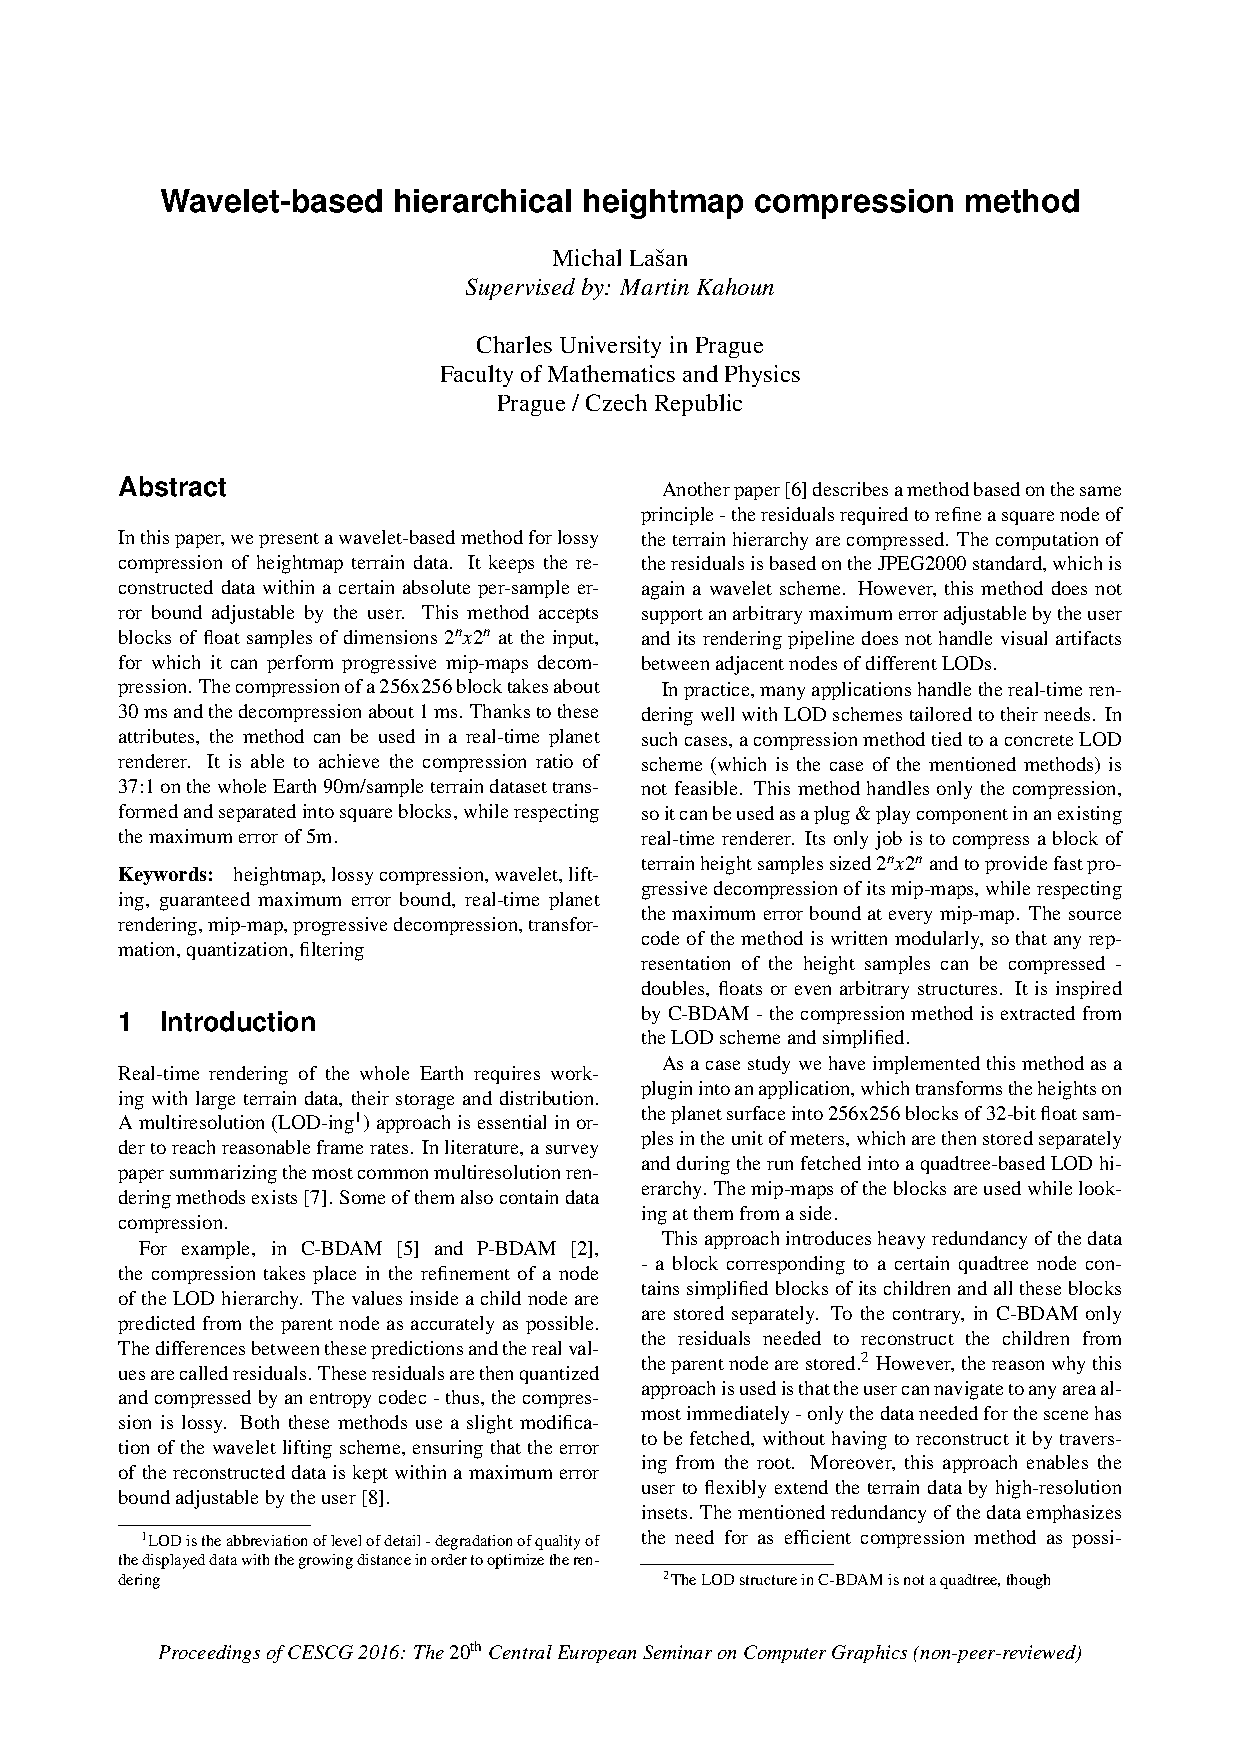
\includepdf[pages=-]{paper.pdf}